\setchapterpreamble[u]{\margintoc}
\chapter{High dimensional statistics and sparsity}
\label{chap:high_dimensional_statistics}

This chapter is about high-dimensional statistics, in particular high-dimensional linear regression, which corresponds to a setting where the sample size $n$ is smaller than the number of features $d$.
Let us consider again the Gaussian linear model (see Chapter~\ref{chap:linear_regression}), where we observe labels satisfying
\begin{equation*}
	Y_i = f(X_i) + \eps_i
\end{equation*}
for $i=1, \ldots, n$, where $X_i \in \R^d$ are vectors of features that we assume deterministic, where $\eps_1, \ldots, \eps_n$ are i.i.d $\nor(0, \sigma^2)$ random variables and where $f$ is the regression function that we want to estimate.


\paragraph{Sparse estimation.}

We consider a set $\cF = \{ f_1, \ldots, f_M \}$ of functions called a \emph{dictionary}, with $M$ which can be much larger than the sample size $n$.  
We want to learn from data an estimator of $f$ of the form
\begin{equation*}
	f_\theta(x) = \sum_{j=1}^M \theta_j f_j(x)
\end{equation*}
with the following properties: the \emph{empirical} estimation error
\begin{equation*}
	\frac 1n \sum_{i=1}^n (f_\theta(X_i) - f(X_i))^2
\end{equation*}
is small and the sparsity of $\theta$, namely
\begin{equation}
	\label{eq:sparsity}
	\norm{\theta}_0 = |J(\theta)| = | \{ j=1, \ldots, M : \theta_j \neq 0\} |,
\end{equation}
where $|J|$ stands for the cardinality of a set $J$, is small compared to~$M$.
If we are able to satisfy both points, we say that we can find a \emph{sparse} linear combination of elements of $\cF$ to estimate $f$.
This task is called \emph{sparse coding} or \emph{sparse estimation}, since it would allow to select a subset of elements from a typically \emph{redundant} dictionary $\cF$ to estimate~$f$.
Of course, if $M = d$ and $f_j(x) = x_j$, we recover the standard linear regression model, where $f_\theta(x) = x^\top \theta$.

Let us introduce a bunch of notations before diving into the main matter.
Here, the features matrix is a $n \times M$ matrix given by
\begin{equation*}
	\bX = 
	\begin{bmatrix}
		f_1(X_1) & \cdots & f_M(X_1) \\
		\vdots & \ddots & \vdots \\
		f_1(X_n) & \cdots & f_M(X_n)
	\end{bmatrix}	
	=
	\begin{bmatrix}
		\bX_1^\top \\
		\vdots \\
		\bX_n^\top 
	\end{bmatrix}
	= 
	\begin{bmatrix}
		\bX^1 \cdots \bX^M
	\end{bmatrix}.
\end{equation*}
Let us introduce also
\begin{equation*}
	\by =
	\begin{bmatrix}
		Y_1 \\
		\vdots \\
		Y_n
	\end{bmatrix},
	\quad
	\bf = 
	\begin{bmatrix}
		f(X_1) \\
		\vdots \\
		f(X_n)
	\end{bmatrix},
	\quad
	\bf_\theta =	
	\begin{bmatrix}
		f_\theta(X_1) \\
		\vdots \\
		f_\theta(X_n)
	\end{bmatrix},
	\quad
	\beps = 
	\begin{bmatrix}
		\eps_1 \\
		\vdots \\
		\eps_n
	\end{bmatrix}.
\end{equation*}
The problem can be rewritten as a Gaussian linear model
\begin{equation*}
	\by = \bX \theta + \beps
\end{equation*}
from Chapter~\ref{chap:linear_regression}, however this time we can have $M \gg n$, namely the matrix $\bX$ can be overdetermined: it is not full-rank, in this case we say that the dictionary $\cF$ is \emph{redundant}.
The notation $\norm{u}$ will stand for the Euclidean norm of $u \in \R^n$.

\paragraph{Oracle inequalities.}

We are looking for an estimator $\wh \theta_n$ such that $\norm{\wh \theta_n}_0 \ll M$ and
\begin{equation}
	\label{eq:oracle-remainder}
	\frac 1n \norm{\bf_{\wh \theta_n} - \bf}^2 
	\leq \inf_{\theta \in \R^M} \Big\{ 
	\frac 1n  \norm{\bf_\theta - \bf}^2 + \remain(\theta) \Big\}
\end{equation}
where $\remain$ is, ideally, a small quantity that depends on $\theta$, but might depend also on $n, \cF$ and $\sigma^2$.
If $\remain$ is small, then such an inequality would prove that the estimator $f_{\wh \theta_n}$ performs almost as well as the best linear combination $f^\star = f_{\theta^\star}$ of elements from $\cF$, where $\theta^\star \in \argmin_{\theta \in \R^M} \norm{\bf_\theta - \bf}^2$.
We say that $f^\star$ is an \emph{oracle}, since it depends on $f$, and an inequality of the form~\eqref{eq:oracle-remainder} is called an \emph{oracle inequality}.

This raises the following questions:
\begin{itemize}
	\item How can we construct a sparse estimator $\wh \theta_n$ ?
	\item What is the value of $\remain$ in the inequality~\eqref{eq:oracle-remainder} ?
\end{itemize}
We will deal with this problem using a penalization which incudes sparsity in $\theta$.
We already talked about the Ridge penalization in Chapter~\ref{chap:bayesian_statistics}, which corresponds to the estimator
\begin{equation}
	\label{eq:chap-lasso-ridge-estimator}
	\wh \theta_n^{\mathsf{ridge}} = \argmin_{\theta \in \R^M} 
	\Big\{ \frac 1n \sum_{i=1}^n (Y_i - f_\theta(X_i))^2 + \frac{\lambda}{2} \norm{\theta}^2 \Big\},
\end{equation}
where $\norm{\theta}$ is the Euclidean norm of $\theta$, also called $\ell_2$-norm.
We proved in Chapter~\ref{chap:bayesian_statistics} that this penalization can be understood as an isotropic Gaussian prior in the Gaussian linear model, and that $\wh \theta_n^{\mathsf{ridge}}$ is the unique solution to the linear system
\begin{equation*}
	(\bX^\top \bX + n \lambda \bI) \theta = \bX^\top \by,
\end{equation*}
which has no obvious reasons of being sparse.
% \todo{Explicit GD sous forme prox}

In this chapter, we will consider another penalization which involves the $\ell_1$ norm, since as explained in what follows, it leads to a simple convex problem which defines a sparse estimator $\wh \theta_n^{\mathsf{lasso}}$, coming from a \emph{convex relaxation} principle.
This estimator is called the \emph{Lasso} (Least Absolute Shrinkage and Selection Operator), introduced in~\sidecite{tibshirani1996regression} and is given by
\begin{equation}
	\label{eq:lasso-def}
		\wh \theta_n^{\mathsf{lasso}} = \argmin_{\theta \in \Theta} 
		\Big\{ \frac 1n \sum_{i=1}^n (Y_i - f_\theta(X_i))^2 + \lambda \norm{\theta}_1 \Big\},
\end{equation}
where $\norm{\theta}_1 = \sum_{j=1}^M |\theta_j|$ is the $\ell_1$ norm of $\theta$ and where $\Theta \subset \R^M$ is a convex set, main examples being
\begin{itemize}
 	\item The whole set $\Theta = \R^M$ (no constraint)
 	\item The set $\Theta = [0, +\infty)^M$ (positivity constraint)
 	\item The set $\theta = [-R, R]^M$ for some $R > 0$ (box constraint)
 \end{itemize}
In order to induce sparsity, it is tempting to use as a penalization the "$\ell_0$ norm", but this leads to a problem where we would need to try out all subsets $J \subset \{ 1, \ldots, M \}$ and train a linear model on each subset of coordinates $J$, which means $2^M$ problems to solve.

\paragraph{Convex relaxation.} % (fold)

The $\ell_1$ can be understood as a \emph{convex relaxation} of $\ell_0$.
Indeed, it is easy to see that the \emph{convex envelope}%
\sidenote{The convex envelope of $g : [a, b] \rightarrow \R$ is, at each point $x \in [a, b]$, the supremum of all convex functions that lie under $g$, namely $g^\text{env}(x) = \sup \{ h(x) : h \text{ convex and } h \leq g \text{ over } [a, b] \} $.}
of the function $g_0(x) = \ind{x \neq 0}$ over the interval $[-1, 1]$ is given by $g_1(x) = |x|$, so that the convex envelope of $x \mapsto \norm{x}_0$ over $[-1, 1]^M$ is $x \mapsto \norm{x}_1$, see Figure~\ref{fig:l0-l1}.
\begin{marginfigure}
	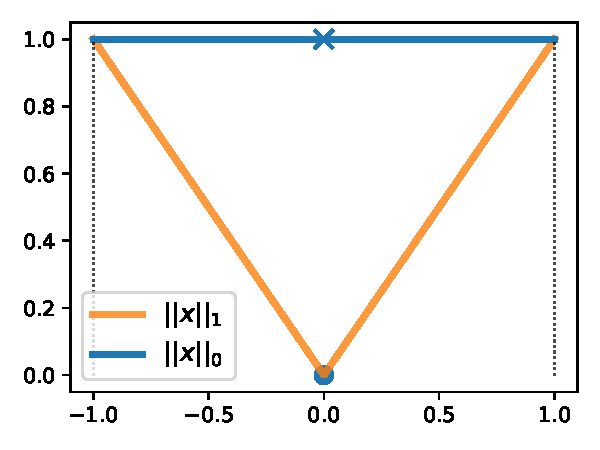
\includegraphics{assets/l0_l1.pdf}
	\caption{The convex envelope of $x \mapsto \norm{x}_0$ over $[-1, 1]$ is $x \mapsto \norm{x}_1$.}
	\label{fig:l0-l1}
\end{marginfigure}
The $\ell_1$ norm therefore appears naturally as a convex relaxation of $\ell_0$.
Another way of understanding it is to consider the following constrained optimization problem
\begin{align*}
	\min \quad &\norm{x}_0 \\ 
	\text{such that} \quad &x \in C \quad \text{and} \quad \norm{x}_\infty \leq R,
\end{align*}
where $C$ is a convex set%
\sidenote{If $C$ is a polyhedron $C : \{ x \in \R^d : \bA x \leq b \}$, then we say that the constraints are \emph{linear}.}
which can be reformulated as
\begin{align*}
	\min \quad &\bone^\top u \\ 
	\text{such that} \quad &u \in \{ 0, 1 \}^M, \quad |x_i| \leq R u_i 
	\quad \text{for all} \quad i=1, \ldots, M \\
	&x \in C
\end{align*}
Such an optimization problem is called a "linear mixed integer program" whenever $C$ is a polyhedron. 
It is hard to solve exactly, since it requires to try out all possible vectors $u \in \{ 0, 1 \}^M$.
% \todo{references}
A convex relaxation of this problem is
\begin{align*}
	\min \quad &\bone^\top u \\ 
	\text{such that} \quad &u \in [0, 1]^M, \quad |x_i| \leq R u_i 
	\quad \text{for all} \quad i=1, \ldots, M \\
	&x \in C
\end{align*}
which can be rewritten as
\begin{align*}
	\min \quad &\frac 1R \norm{x}_1 \\ 
	\text{such that} \quad &x \in C \quad \text{and} \quad \norm{x}_\infty 
	\leq R,
\end{align*}
where we see that, once again, the $\ell_1$ norm naturally appears.

% \todo{Laplace Prior}

\paragraph{Soft-thresholding.}

A straightforward computation allows to understand that the $\ell_1$ norm induces sparsity.
Indeed, we can see easily that
\begin{equation}
	\label{eq:soft-thresholding1}
	\argmin_{a \in \R} \{ \frac12 (a - b)^2 + \lambda |a| \Big\} 
	= \sign(b) (|b| - \lambda)_+
\end{equation}
for any $b \in \R$, where $x_+ = \max(x, 0)$ and $\sign(x) = 1$ if $x > 0$, $\sign(x) = -1$ if $x < 0$ and $\sign(0) = 0$.
This proves that
\begin{equation}
	\label{eq:soft-thresholding2}
	\argmin_{a \in \R^M} \Big\{ \frac12 \norm{a - b}_2^2 + \lambda \norm{a}_1 \Big\}
	= T_\lambda(b)
\end{equation}
for any $b \in \R^M$, where $T_\lambda : \R^M \rightarrow \R^M$ is the \emph{soft-thresholding} operator given by 
\begin{equation*}
	(T_\lambda(b))_j = \sign(b_j) (|b_j| - \lambda)_+
\end{equation*}
for $j=1, \ldots, M$, see Figure~\ref{fig:soft-thresholding}.
We display also in Figure~\ref{fig:soft-thresholding} the \emph{shrinkage} operator $(S_\lambda(b))_j = b_j / (1 + \lambda)$, which corresponds to the Ridge penalization, since $\argmin_{a \in \R} \{ (a - b)^2 + \lambda a^2 \} = b / (1 + \lambda)$.
\begin{marginfigure}
	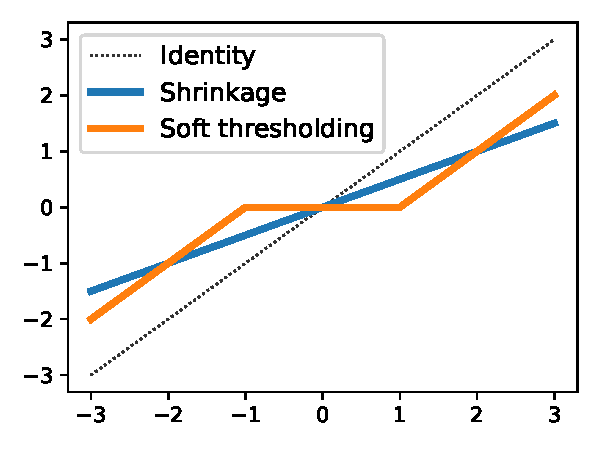
\includegraphics{assets/soft_thresholding.pdf}
	\caption{Soft-thresholding and shrinkage with $\lambda = 1$ on a single coordinate.}
	\label{fig:soft-thresholding}
\end{marginfigure}

% % \todo{descente de gradient proximale}

We observe that the shrinkage operator, which corresponds to the Ridge penalization, does not induce sparsity, while soft-thresholding does.
The fact that the $\ell_1$ norm induces sparsity (coordinates can be 0) actually comes from the fact that the absolute value is not differentiable at $0$.
It can be understood geometrically as well, using the fact that a unit $\ell_1$ ball has sparse corners at $\pm e_j$ for $j=1, \ldots, M$ (canonical basis vectors) that are \emph{sparse} vectors: when we project a point onto an $\ell_1$ ball, we are likely to project onto a corner or an edge, that are sets of sparse points.
\begin{marginfigure}
	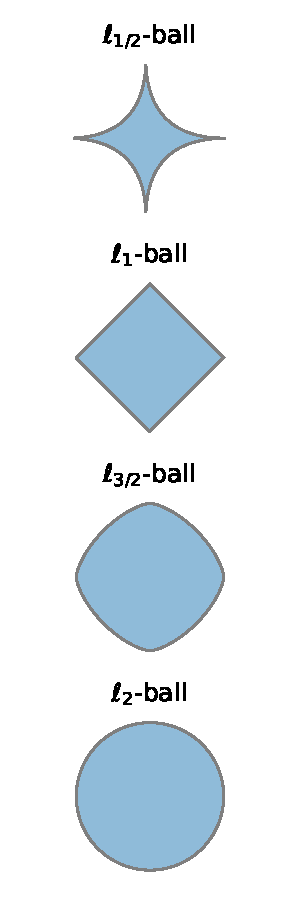
\includegraphics{assets/balls.pdf}
	\caption{Some $\ell_p$ balls in $\R^2$. The $\ell_1$ ball is convex but has spiky corners}
	\label{fig:balls}
\end{marginfigure}

% Pour la boule L1 3D, voir https://plotly.com/python/3d-mesh/
% https://stackoverflow.com/questions/9170838/surface-plots-in-matplotlib
% https://jakevdp.github.io/PythonDataScienceHandbook/04.12-three-dimensional-plotting.html


The discussion above motivates the use of the $\ell_1$ norm to induce sparsity.
Let us therefore consider the estimator $\wh \theta_n^{\mathsf{lasso}}$ given by~\eqref{eq:lasso-def}, that we will simply denote $\wh \theta_n$ in the rest of the chapter.
In order to study the statistical properties of this estimator, we need some tools from convex optimization.

% \todo{This estimator is called the Lasso BLABLA + reference + reference francis + expliciter l'optimisation par descente de gradient, descente de gradient par coordonnees}

% \todo{Chemin regularization du Lasso}

\section{Some tools from convex optimization} % (fold)
\label{sec:some_tools_from_convex_optimization}

Let us consider a convex function $\phi : \R^d \rightarrow \R$.
A fundamental notion which generalizes the differential to non-differentiable convex functions is the \emph{subdifferential}, see Figure~\ref{fig:subdifferential}.
\begin{marginfigure}
	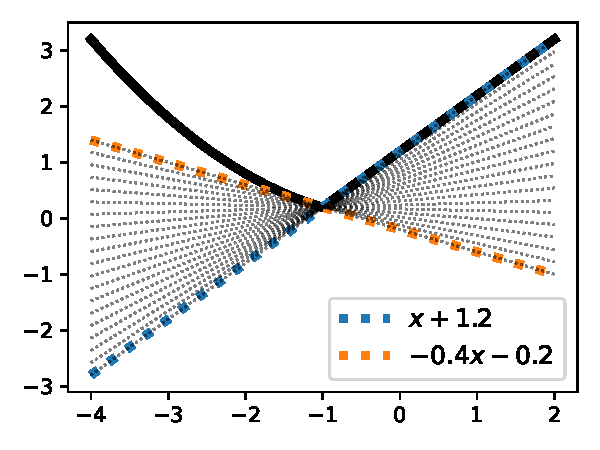
\includegraphics{assets/subdifferential.pdf}
	\caption{An illustration of the subgradients of a convex function at $x=-1$. The subdifferential is equal to the interval $[-0.4, 1]$.}
	\label{fig:subdifferential}
\end{marginfigure}
\begin{definition}
	\label{def:subdifferential}
	We say that $g \in \R^d$ is a \emph{subgradient} of a convex function $\phi : \R^d \rightarrow \R$ at $u \in \R^d$ if and only if
	\begin{equation}
	 	\phi(v) - \phi(u) \geq g^\top (v - u)
	 \end{equation} 
	 for any $v \in \R^d$.
	 The set of all subgradients
	 \begin{equation*}
	 	\partial \phi(u) = \big\{ g \in \R^d : \phi(v) - \phi(u) \geq g^\top (v -u) 
	 	\; \text{ for all } \; v \in \R^d \}
	 \end{equation*}
	 is called the \emph{subdifferential} of $\phi$ at $u$.
\end{definition}
An example is with $\phi(u) = |u|$, where we have $\partial \phi(u) = \{ 1 \}$ if $u > 0$, $\partial \phi(u) = \{ -1 \}$ if $u < 0$ and $\partial \phi(u) = [-1, 1]$ if $u = 0$.
Whenever $\phi$ is differentiable at $u$, we have obviously that $\partial \phi(u) = \{  \grad \phi(u) \}$.
Another obvious claim is that
% \sidenote{TODO: proof}
\begin{equation*}
	u^\star \in \argmin_{u \in \R^d} \phi(u) \quad \text{if and only if} \quad 0 \in \partial \phi(u^\star).
\end{equation*}
Also, it is easy to see that
\begin{equation*}
	\partial \Big( \sum_{k=1}^K \alpha_k \phi_k(u) \Big) = \sum_{k=1}^K \alpha_k \partial \phi_k(u)
\end{equation*}
whenever $\alpha_k \geq 0$ and $\phi_k$ are convex functions for all $k=1, \ldots, K$.
Another nice formula allows to express the subdifferential of a maximum of convex functions with the subdifferential of each function.
Indeed, if $\phi(u) = \max_{k=1}^K \phi_k(u)$, we have
\begin{equation}
	\label{eq:subdifferential-max}
	\partial \phi(u) = \conv\Big( \bigcup_{k=1}^K \Big\{ \partial \phi_k(u) : \phi_k(u) = \phi(u) \Big\} \Big),
\end{equation}
where $\conv(A)$ stands for the convex hull of a set $A$.
For instance, if $\phi_1 : \R \rightarrow \R$ and $\phi_2 : \R \rightarrow \R$ are convex and differentiable functions, we have%
\begin{marginfigure}[*-3]
	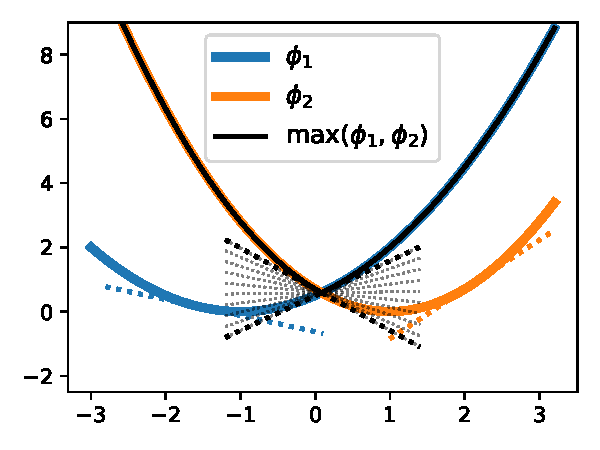
\includegraphics{assets/subdifferential-max.pdf}
	\caption{An illustration of formula~\eqref{eq:subdifferential-max-1D}.}
	\label{fig:subdifferential-max}
\end{marginfigure}
\begin{equation}
	\label{eq:subdifferential-max-1D}
	\partial \max(\phi_1, \phi_2)(u) = 
	\begin{cases}
	\{ \phi_2'(u) \} &\text{ if } \phi_2(u) > \phi_1(u) \\
	\{ \phi_1'(u) \} &\text{ if } \phi_2(u) < \phi_1(u) \\
	[ \phi_1'(u), \phi_2'(u) ] &\text{ if } \phi_2(u) = \phi_1(u) \\
	\end{cases}
\end{equation}
Another useful definition is the indicator function of a convex set $C \subset \R^d$
\begin{equation*}
	\delta_C(u) = \begin{cases}
		0 &\text{if } u \in C \\
		+\infty &\text{if } u \notin C.
	\end{cases}
\end{equation*}
If allows to reformulate a \emph{constrained} problem as an \emph{unconstrained} one, namely to rewrite
\begin{equation*}
	u^\star \in \argmin_{u \in C} \phi(u) \quad \text{ as } \quad u^\star \in \argmin_{u \in \R^d} \{ \phi(u) + \delta_C(u) \}
\end{equation*}
which means that $0 \in \partial \phi(u^\star) + \partial \delta_C(u^\star)$, namely that there is $g^\star \in \partial \phi(u^\star)$ such that $-g^\star \in \partial \delta_C(u^\star)$.
But it is easy to understand what the subdifferential of the indicator function $\delta_C$ is, since $g \in \partial \delta_C(u^\star)$ with $u^\star \in C$ means%
\sidenote{using the definition of the subdifferential}
that
\begin{equation*}
	\delta_C(u) - \delta_C(u^\star) \geq g^\top (u - u^\star) \quad \text{for all} \quad u \in \R^d,
\end{equation*}
but $\delta_C(u^\star) = 0$ so that, for any $u \in C$, we have
\begin{equation*}
	\partial \delta_C(u) = \big\{ g \in \R^d : g^\top (v - u) \leq 0 \quad 
	\text{ for all } v \in C \big\},
\end{equation*}
which is the \emph{normal cone} to $C$ at $u$, see Figure~\ref{fig:normal-cone}.
\begin{marginfigure}[*-3]
	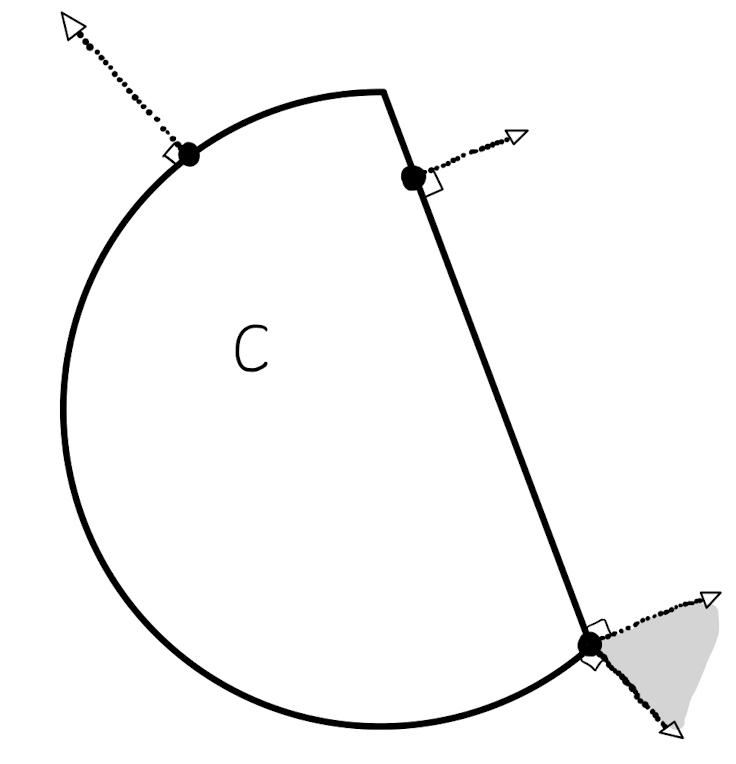
\includegraphics{assets/normal-cone.png}
	\caption{Illustration of normal cones}
	\label{fig:normal-cone}
\end{marginfigure}
This proves the following proposition.
\begin{proposition}
	\label{prop:optimality-criterion}
	Let $\phi : \R^d \rightarrow \R$ be a convex function and $C \subset \R^d$ be a convex set. 
	An optimality criterion for the problem
	\begin{equation*}
		u^\star \in \argmin_{u \in C} \phi(u)
	\end{equation*}
	is given by
	\begin{equation*}
		\exists g^\star \in \partial \phi(u^\star) \quad \text{such that} 
		\quad (g^\star)^\top (u - u^\star) \geq 0
	\end{equation*}
	for all $u \in C$, where $\partial \phi(u^\star)$ is the subdifferential of $\phi$ at $u^\star$.
\end{proposition}
%\todo{j'ai un moins devant dans mes note}

Another property about the subdifferential is the following.
\begin{proposition}[Monotonicity of the subdifferential]
	Given a convex function $\phi : \R^d \rightarrow \R$, any $u_1, u_2 \in \R^d$ and any $g_1 \in \partial \phi(u_1)$ and $g_2 \in \partial \phi(u_2)$, we have
	\begin{equation*}
		(u_1 - u_2)^\top (g_1 - g_2) \geq 0.
	\end{equation*}
\end{proposition}
The proof is straightforward.%
\sidenote{Just use Definition~\ref{def:subdifferential} to write that $\phi(u_2) - \phi(u_1) \geq g_1^\top(u_2 - u_1)$ and that $\phi(u_1) - \phi(u_2) \geq g_2^\top(u_1 - u_2)$ and add the two.}

\paragraph{Subdifferential of $\ell_1$ norm.} 

Let us give as an example the computation of the subdifferential of the $\ell_1$ norm.
Put $\phi(u) = \norm{u}_1$ and note that it can be rewritten as
\begin{equation*}
	\norm{u}_1 = \max \big\{ e^\top u : e \in \{ -1, 1 \}^d \big\} = \max_{i=1, \ldots, 2^d} \phi_i(u)
\end{equation*}
where we introduced $\phi_i(u) = e_i^\top u$ for $e_1, \ldots, e_{2^d}$ the elements of $\{ -1, 1 \}^d$.
Note that given $u \in \R^d$, we can choose $e(u) \in \R^d$ such that $e(u)_j = 1$ if $u_j > 0$, $e(u)_j = -1$ if $u_j < 0$ and $e(u)_j = 1$ \emph{or} $e(u)_j = -1$ if $u_j = 0$, in order to obtain that $e(u)^\top u = \norm{u}_1$.
Let us introduce the set
\begin{equation*}
	I(u) = \big\{ i \in \{ 1, \ldots 2^d \} : e_i^\top u = \norm{u}_1 \big\}.
\end{equation*}
Each function $\phi_i$ is differentiable and $\grad \phi_i(u) = e_i$. 
So, we can apply Equation~\eqref{eq:subdifferential-max} to obtain that
\begin{equation}
	\label{eq:subdifferential-l1}
	\begin{split}
	\partial \norm{u}_1 &= \conv\Big( \bigcup_{i \in I(u)} \{ e_i \} \Big) \\
	&= \big\{ \sign(u) + h : h \in \R^d, \; \norm{h}_\infty \leq 1, \; h \odot u = 0 
	\big\},
	\end{split}
\end{equation}
where $h \odot u$ is the Hadamard product given by $(h \odot u)_j = h_j u_j$.
For instance if $d = 4$ and $u = [17 \; -42 \; 0 \; 3]^\top$ then $\partial \norm{u}_1 = \{ 1 \} \times \{ -1 \} \times [-1, 1] \times \{ 1 \}$.

\section{Oracle inequalities for the Lasso} % (fold)

The material used in this Section is based on~\sidecite{bickel2009,koltchinskii2011}.
Also, a very nice broader book on the topic of high-dimensional statistics is~\cite{giraud2014introduction}.
Throughout the section, we will assume that the columns are standardized, namely that $\norm{\bX^j}_2 = \sqrt n$.
This is a rather unrestrictive assumption (we could do without it) that follows good-practice when using linear methods in machine learning.
Let us recall that the Lasso estimator is given by
\begin{equation}
	\label{eq:lasso-def-oracle-sec}
	\begin{split}
	\wh \theta_n &= \argmin_{\theta \in \Theta} \Big\{ \frac 1n \sum_{i=1}^n (Y_i - f_\theta(X_i))^2 + \lambda \norm{\theta}_1 \Big\} \\
	&= \argmin_{\theta \in \Theta} \Big\{ 
	\frac 1n \norm{\by - \bf_\theta}^2 + \lambda \norm{\theta}_1 
	\Big\},
	\end{split}
\end{equation}
for some convex set $\Theta \subset \R^M$, where 
\begin{equation*}
	\lambda = 2 \sigma \sqrt{\frac{2(x + \log M)}{n}}
\end{equation*}
with $x > 0$ which corresponds to a confidence level (see Theorem~\ref{thm:oracle-slow} and~\ref{thm:oracle-fast} below) and with $\sigma > 0$ the standard-deviation of the noise.
%  \todo{notation pour $\bf$ et autres}
\begin{theorem}
	\label{thm:oracle-slow}
	If $\wh \theta_n$ is given by~\eqref{eq:lasso-def-oracle-sec}, we have that
	\begin{equation*}
		\frac 1n \norm{\bf_{\wh \theta_n} - \bf}^2 \leq \inf_{\theta \in \Theta} 
		\Big\{ \frac 1n \norm{\bf_{\theta} - \bf}^2  + 2 \lambda \norm{\theta}_1 \Big\}
	\end{equation*}
	with a probability larger than $1 - 2 e^{-x}$.
\end{theorem}
This inequality is called a \emph{slow oracle inequality} since the remainder is $O(1 / \sqrt{n})$.
The proof of Theorem~\ref{thm:oracle-slow} is given in Section~\ref{sec:lasso-proofs} below.
In order to obtain a faster $O(1 / n)$ rate, we need an extra assumption on the matrix of features $\bX$.
Let us introduce the $M \times M$ matrix 
\begin{equation*}
	\bG = \frac 1n \bX^\top \bX = 
	\Big[ \frac 1n \inr{\bf_j, \bf_{j'}} \Big]_{1 \leq j, j' \leq M},
\end{equation*}
where $\bf_j = [f_j(X_1) \cdots f_j(X_n)] \in \R^n$ and $\inr{\cdot, \cdot}$ is the inner product on $\R^n$.
Note that if $M > n$, we have that
\begin{equation*}
	\min_{t \in \R^M \setminus \{ 0 \}} \frac{\sqrt{t^\top \bG t}}{\norm{t}} 
	= \min_{t \in \R^M \setminus \{ 0 \}} \frac{\norm{\bX t}}{\sqrt n \norm{t}} = 0
\end{equation*}
since $\bX : \R^M \rightarrow \R^n$ and $\ker(\bX) \neq \{ 0 \}$ hence the smallest eigenvalue of $\bG$ is zero.

The assumption we are going to use requires that the smallest eigenvalue \emph{restricted} to \emph{sparse} vectors is positive.
For $\theta \in \R^M$ and $c_0 > 0$, let us introduce the cone
\begin{equation}
	\label{eq:def-cone-C}
	C_{\theta, c_0} = \big\{ t \in \R^M : \norm{t_{J(\theta)^\complement}}_1 
	\leq c_0 \norm{t_{J(\theta)}}_1 \big\},
\end{equation}
where
\begin{itemize}
	\item $J(\theta) = \{ j \in \{1, \ldots, M\} : \theta_j \neq 0 \}$ is the 
	\emph{support} of $\theta$,
	\item $t_J \in \R^M$ stands for the vector with coordinates $(t_J)_j = t_j$ if $j \in J$ and $(t_J)_j = 0$ for $j \notin J$,
	\item $J^\complement = \{ 1, \ldots, M \} \setminus J$.
\end{itemize}
If $t \in C_{\theta, c_0}$, then both the vectors $t$ and $\theta$ almost share the same support, since the coefficients of $t_{J(\theta)}$ dominate those of $t_{J(\theta)^\complement}$.
Then, we can introduce 
\begin{equation}
	\label{eq:def-mu-re}
	\mu_{c_0}(\theta) = \inf \Big\{ \mu > 0 : 
	\norm{t_{J(\theta)}} \leq \frac{\mu}{\sqrt n} \norm{\bX t} 
	\; \text{ for all } \; t \in C_{\theta, c_0} \Big\}.
\end{equation}
Note that the function $c_0 \mapsto \mu_{c_0}(\theta)$ is decreasing.
If $c_0 = \infty$, then $C_{\theta, c_0} = \R^M$, while if $c_0 = 0$ then
$C_{\theta, c_0} = \{ t \in \R^M : J(t) = J(\theta) \}$ and in this case
\begin{equation*}
	\mu_{c_0}(\theta) 
	= \frac{1}{\lambda_{\min}(\bG_{J(\theta) \times J(\theta)})^{1/2}}
\end{equation*}
the square-root of the inverse of the smallest eigenvalue of the submatrix $(\bG)_{J \times J}$ with $J = J(\theta)$ corresponding to the subset of rows and columns with index in $J$.
\begin{theorem}
	\label{thm:oracle-fast}
	If $\wh \theta_n$ is given by~\eqref{eq:lasso-def-oracle-sec} where we replace $\lambda$ by $2 \lambda$, we have that
	\begin{align*}
		\frac 1n &\norm{\bf_{\wh \theta_n} - \bf}^2 \\
		&\leq \inf_{\theta \in \Theta} 
		\bigg\{ \frac 1n  \norm{\bf_{\theta} - \bf}^2  + 18 \mu_3(\theta)^2 \sigma^2 \frac{x + \log M}{n} \norm{\theta}_0 \bigg\}
	\end{align*}
	with a probability larger than $1 - 2 e^{-x}$, where $\mu_3(\theta)$ is given by~\eqref{eq:def-mu-re} with $c_0 = 3$ and $\norm{\theta}_0$ is the sparsity of $\theta$ given by~\eqref{eq:sparsity}.
\end{theorem}
The proof of Theorem~\ref{thm:oracle-fast} is given in Section~\ref{sec:lasso-proofs} below.
It proves that the Lasso estimator $\wh \theta_n$ realizes a balance between an \emph{approximation} or \emph{estimation} term $\norm{\bf_{\theta} - \bf}^2$ and a \emph{complexity} term which involves  the sparsity of $\theta$.

It is a remarkable theorem, since it shows that the Lasso estimator, which is the solution of a simple convex problem, is almost as good as the best \emph{sparse} representation of $f$ using the dictionary $\cF$.
Indeed, the rate obtained herein is of order $(\log M) \norm{\theta}_0 / n$, namely the ambient dimension $M$ appears only through $\log M$, while $\norm{\theta}_0$ corresponds to the "useful" dimension given by the number of elements of $\cF$ that are statistically useful to estimate $f$.
\begin{definition}[Restricted eigenvalues]
	We say that $\bX$ satisfies the $\text{RE}(s, c_0)$ assumption for some $c_0 > 0$ and some $s \in \{ 1, \ldots, M \}$ whenever
	\begin{equation*}
		\kappa(s, c_0) = 
		\min_{\substack{J \subset \{ 1, \ldots, M \} \\ 
			  |J| \leq s}}
			\;
		\min_{\substack{t \neq 0 \\ 
		\norm{t_{J^\complement}}_1 \leq c_0 \norm{t_J}_1}}
		\frac{\norm{\bX t}}{\sqrt n \norm{t_J}} > 0.
	\end{equation*}
\end{definition}
Note that we have
\begin{equation*}
	\kappa(s, c_0) = \inf_{\substack{t \in \R^M \setminus \{ 0 \}\\ 
	\norm{t}_0 \leq s}}
	\; \frac{1}{\mu_{c_0}(t)}.
\end{equation*}
Moreover, whenever $\bX$ satisfies $\text{RE}(s, 1)$, any sub-matrix of $\bX$ formed by any subset of $2 s$ columns from $\bX$ has full rank.%
\sidenote{Suppose by contradiction that there is $t \in \R^M$ such that $\norm{t}_0 = 2s$ and $\bX t = 0$. Then, we can choose disjoint sets $J_0, J_1 \subset \{ 1, \ldots, M\}$ such that $J(t) = J_0 \cup J_1$ with $|J_0| = s$ and $|J_1| = s$ and such that $\norm{t_{J_1}}_1 \leq \norm{t_{J_0}}_1$. 
But obviously $\norm{t_{J_1}}_1 = \norm{t_{J_0^\complement}}_1$ so $\norm{t_{J_0^\complement}}_1 \leq \norm{t_{J_0}}_1$, which contradicts the $\text{RE}(s, 1)$ assumption.}

An immediate corollary of Theorem~\ref{thm:oracle-fast} is the following oracle inequality, which holds under the $\text{RE}(s, 3)$ assumption:
\begin{equation*}
	\frac 1n \norm{\bf_{\wh \theta_n} - \bf}^2 \leq 
	\inf_{\substack{\theta \in \Theta \\ \norm{\theta}_0 \leq s}}
	\bigg\{ \frac 1n  \norm{\bf_{\theta} - \bf}^2  + \frac{18 \sigma^2}{\kappa(s, 3)^2} 
	\; \frac{s(x + \log M)}{n} \bigg\}
\end{equation*}
with a probability larger than $1 - e^{-x}$.
In this inequality, the convergence rate is of order $(s \log M) / n$, where $s$ is the sparsity of the best $\theta$.
Let us finish this chapter with several remarks before diving into the proofs.
\begin{itemize}
	\item The rate of convergence depends on the ambient dimension $M$ only through $\log M$ and depends linearly on the sparsity $s$ of $\theta \in \R^M$. This is a remarkable property called \emph{dimension reduction} or \emph{adaptation to the sparsity} of the Lasso estimator.
	\item This is not the optimal rate, the minimax optimal rate among $s$-sparse vector (and in a $\ell_q$ ball) being $s \log(M / s) / n$, see~\sidecite{verzelen2012}.
	\item There are several improvements of these oracle inequalities in literature: beyond Gaussian noise, using the integrated estimator error $\int_{\R^M} (f_{\wh \theta_n}(x) - f(x))^2 P_X(dx)$ instead of the empirical one used here, and we can remove the dependency of $\lambda$ on the confidence level $x > 0$.
	\item From Theorem~\ref{thm:oracle-fast}, we can derive bounds on the estimator error $\norm{\wh \theta_n - \theta^\star}_p$ (measured by the $\ell_p$ norm, $p \geq 1$) of the true parameter $\theta^\star$ and the we can give guarantees on the \emph{signed support recovery} of the parameter, through controls on the probability 
	$\P[ \sign(\wh \theta_n) = \sign(\theta^\star)]$, see~\sidecite{zhao2006model}.
\end{itemize}

\section{Proofs} % (fold)
\label{sec:lasso-proofs}


\subsection{Proof of Theorem~\ref{thm:oracle-slow}} % (fold)
\label{sub:proof_of_theorem_thm:oracle-slow}

Let us start with the noise. It is fairly easy, since
\begin{align*}
	\frac 1n \sum_{i=1}^n \eps_i f_j(X_i) 
	&\sim \nor\Big( 0, \frac{\sigma^2}{n^2} \sum_{i=1}^n f_j(X_i)^2 \Big) \\
	&= \nor\Big( 0, \frac{\sigma^2}{n^2} \norm{\bX_j}^2 \Big) \\
	\marginnote{We assumed that $\norm{\bX_j} = \sqrt n$}
	&= \nor\Big( 0, \frac{\sigma^2}{n} \Big).
\end{align*}
So, recalling that $\P[|Z| \geq z] \leq 2e^{-z^2 / 2}$ whenever $Z \sim \nor(0, 1)$ for any $z > 0$,%
% \todo{insert side proof}
we obtain
\begin{equation*}
	\P \bigg[ \Big| \frac 1n \sum_{i=1}^n \eps_i f_j(X_i) \Big| \geq \sigma \sqrt{\frac{2 x}{n}} \bigg] \leq 2 e^{-x}
\end{equation*}
and using an union bound, we obtain that the event
\begin{equation*}
	A = \bigcap_{j=1}^M \bigg\{ \Big| \frac 1n \sum_{i=1}^n \eps_i f_j(X_i) \Big| \leq \sigma \sqrt{\frac{2 (x + \log M)}{n}} \bigg\}
\end{equation*}
satisfies $\P[A] \geq 1 - 2e^{-x}$.
The definition of $\wh \theta$ entails that
\begin{equation}
	\label{eq:proof-oracle-slow-step1}
	\frac 1n  \norm{\by - \bf_{\wh \theta}}^2 + \lambda \norm{\wh \theta}_1 
	\leq \frac 1n  \norm{\by - \bf_\theta}^2 + \lambda \norm{\theta}_1
\end{equation}
for any $\theta \in \Theta$ and an easy computation gives
\begin{equation}
	\label{eq:proof-oracle-slow-step2}
	\begin{split}
	&\frac 1n \norm{\by - \bf_{\wh \theta}}^2 - \frac 1n \norm{\by - \bf_\theta}^2 \\
	&= \frac 1n  \norm{\bf_{\wh \theta}}^2 + \frac 1n  \norm{\bf}^2 + \frac 2n  \inr{\by, \bf_{\theta} - \bf_{\wh \theta}} \\
	&= \frac 1n \norm{\bf_{\wh \theta}}^2 + \frac 1n \norm{\bf}^2 + \frac 2n  \inr{\bf, \bf_{\theta} - \bf_{\wh \theta}} + \frac 2n  \inr{\beps, \bf_{\theta} - \bf_{\wh \theta}} \\
	&= \frac 1n \norm{\bf_{\wh \theta} - \bf}^2 - \frac 1n \norm{\bf_\theta - \bf}^2 + 
	\frac 2n  \inr{\beps, \bf_{\theta} - \bf_{\wh \theta}}.
	\end{split}
\end{equation}
But on the event $A$, we have that
\begin{equation}
	\label{eq:proof-oracle-slow-step3}
	\begin{split}
	\frac 2n | \inr{\beps, \bf_{\theta} - \bf_{\wh \theta}} | 
	&= \Big| \frac 2n \sum_{j=1}^M (\wh \theta_j - \theta_j ) 
	\sum_{i=1}^n \eps_i f_j(X_i) \Big| \\
	&\leq \sum_{j=1}^M | \wh \theta_j - \theta_j | 2 \sigma \sqrt{\frac{2 (x + \log M)}{n}} \\
	&= \lambda \norm{\wh \theta - \theta}_1,	
	\end{split}
\end{equation}
so that, combining Inequalities~\eqref{eq:proof-oracle-slow-step1},~\eqref{eq:proof-oracle-slow-step2} and~\eqref{eq:proof-oracle-slow-step3}, we end up with
\begin{align*}
	\frac 1n \norm{\bf_{\wh \theta} - \bf}^2 &
	\leq \frac 1n \norm{\bf_\theta - \bf}^2 
	+ \lambda \norm{\wh \theta - \theta}_1 
	+ \lambda \norm{\theta}_1 
	- \lambda \norm{\wh \theta}_1 \\
	&\leq \frac 1n \norm{\bf_\theta - \bf}^2 + 2 \lambda \norm{\theta}_1,
\end{align*}
which concludes the proof of Theorem~\ref{thm:oracle-slow}. $\hfill \square$


\subsection{Proof of Theorem~\ref{thm:oracle-fast}} % (fold)
\label{sub:proof_of_theorem_thm:oracle-fast}

% \todo{attention au facteur 2 devant la penalisation}

Let us recall that we study the estimator
\begin{equation}
	\label{eq:lasso-def-proof}
	\wh \theta \in \argmin_{\theta \in \Theta} \big\{ R_n(\theta) + 2 \pen(\theta) \big\},
\end{equation}
where $\Theta \subset \Theta$ is a convex set, where 
\begin{equation*}
	R_n(\theta) = \frac 1n \sum_{i=1}^n (Y_i - f_\theta(X_i))^2	
	= \frac 1n \norm{\by - \bf_{\theta}}^2
\end{equation*}
is convex and differentiable and $\pen(\theta) = \lambda \norm{\theta}_1$ is convex.
We have $\grad R_n(\theta) = - \frac 2n \bX^\top (\by - \bX \theta)$ so that
\begin{equation*}
	\partial(R_n + \pen)(\theta) = - \frac 2n \bX^\top (\by - \bX \theta) + 2 \lambda 
	\partial \norm{\theta}_1.
\end{equation*}
Using Proposition~\ref{prop:optimality-criterion}, we have that~\eqref{eq:lasso-def-proof} is equivalent to the fact that there is $\wh g \in \partial \norm{\wh \theta}_1$ such that
\begin{equation}
	\label{eq:lasso-proof-cond1}
	\Big \langle - \frac 2n \bX^\top (\by - \bX \wh \theta) + 2 \lambda \wh g, \wh \theta - \theta \Big \rangle \leq 0 \quad \text{for all} \quad \theta \in \Theta.
\end{equation}
Let us choose for now an arbitrary $\theta \in \Theta$ and note $J = J(\theta)$.
We can rewrite inequality~\eqref{eq:lasso-proof-cond1} as
\begin{equation*}
	\frac 2n \big \langle  \bX^\top \bX \wh \theta, \wh \theta - \theta \big \rangle 
	- \frac 2n \big \langle \bX^\top \by, \wh \theta - \theta \big \rangle
	+ 2 \lambda \inr{\wh g, \wh \theta - \theta} \leq 0,
\end{equation*}
and, recalling that $\bX \theta = \bf_\theta$ and that $\by = \bf + \beps$, we have
\begin{align*}
	\frac 2n \langle \bf_{\wh \theta}, \bf_{\wh \theta} &- \bf_{\theta} \rangle 
	- \frac 2n  \inr{\bf,  \bf_{\wh \theta} - \bf_\theta} \\
	&- \frac 2n \inr{\beps, \bf_{\wh \theta} - \bf_\theta}
	+ 2 \lambda \inr{\wh g, \wh \theta - \theta} \leq 0,
\end{align*}
that we can rewrite as 
\begin{align*}
	\frac 2n \inr{ \bf_{\wh \theta} - \bf, \bf_{\wh \theta} - \bf_{\theta}}
	&+ 2 \lambda  \inr{\wh g - g, \wh \theta - \theta} \\
	\leq &- 2 \lambda  \inr{g, \wh \theta - \theta} 
	+ \frac 2n  \inr{\beps,  \bf_{\wh \theta} - \bf_\theta} 
\end{align*}
for any $g \in \partial \norm{\theta}_1$. 
But, the monotonicity of the subdifferential entails that $\inr{\wh g - g, \wh \theta - \theta} \geq 0$ and and easy computation gives (Al-Kachi)
\begin{equation*}
	2 \inr{ \bf_{\wh \theta} - \bf, \bf_{\wh \theta} - \bf_{\theta}} 
	= \norm{\bf_{\wh \theta} - \bf_{\theta}}^2 
	+ \norm{\bf_{\wh \theta} - \bf}^2
	- \norm{\bf_{\theta} - \bf}^2
\end{equation*}
so that we end up with
\begin{align*}
	\frac 1n \norm{\bf_{\wh \theta} - \bf}^2 &
	+ \frac 1n \norm{\bf_{\wh \theta} - \bf_{\theta}}^2 \\
	&\leq \frac 1n \norm{\bf_{\theta} - \bf}^2
    - 2 \lambda \inr{g, \wh \theta - \theta} 
	+ \frac 2n  \inr{\beps,  \bf_{\wh \theta} - \bf_\theta}.
\end{align*}
for any $g \in \partial \norm{\theta}_1$.
Now, we need to use what the subdifferential of the $\ell_1$ norm is.
Using~\eqref{eq:subdifferential-l1}, we can write $g = \sign(\theta) + h$ for any $h$ such that where $h_J = 0$ and $\norm{h}_\infty \leq 1$.
We have 
\begin{equation*}
	|\inr{\sign(\theta), \wh \theta - \theta}| = |\inr{\sign(\theta), (\wh \theta - \theta)_J}| \leq \norm{(\wh \theta - \theta)_J}_1.
\end{equation*}
and we can choose $h$ such that
\begin{equation*}
	\inr{h, \wh \theta - \theta} = \inr{h, \wh \theta_{J^\complement}} 
	= \norm{\wh \theta_{J^\complement}}_1 
	= \norm{(\wh \theta - \theta)_{J^\complement}}_1.
\end{equation*}
This leads to
\begin{align*}
	\frac 1n \norm{\bf_{\wh \theta} - \bf}^2 &+ \frac 1n \norm{\bf_{\wh \theta} - \bf_{\theta}}^2
	+ 2 \lambda \norm{\wh \theta_{J^\complement}}_1 \\
	&\leq \frac 1n \norm{\bf_{\theta} - \bf}^2
    + 2 \lambda \norm{(\wh \theta - \theta)_J}_1
	+ \frac 2n  \inr{\beps,  \bf_{\wh \theta} - \bf_\theta}.
\end{align*}
If $\norm{\bf_{\wh \theta} - \bf}^2 + \norm{\bf_{\wh \theta} - \bf_{\theta}}^2 - \norm{\bf_{\theta} - \bf}^2 \leq 0$, then $\norm{\bf_{\wh \theta} - \bf}^2 \leq \norm{\bf_{\theta} - \bf}^2$, which concludes the proof, so let us consider from now on the other case, which entails that
\begin{equation}
	\label{eq:lasso-proof-on-A}
	2 \lambda \norm{\wh \theta_{J^\complement}}_1 
	\leq 2 \lambda \norm{(\wh \theta - \theta)_J}_1
	+ \frac 2n  \inr{\beps,  \bf_{\wh \theta} - \bf_\theta}.
\end{equation}
On the event $A$,%
\sidenote{see the proof of Theorem~\ref{thm:oracle-slow}}
we have $\frac 1n \norm{\bX^\top \beps}_\infty \leq \lambda / 2$ where we recall that $\lambda = 2 \sigma \sqrt{2 (x + \log M) / n}$.
This entails 
\begin{align*}
	\frac 2n \inr{\beps,  \bf_{\wh \theta} - \bf_\theta} &=
	\frac 2n \inr{\bX^\top \beps, \wh \theta - \theta} \\
	&= \frac 2n \inr{\bX^\top \beps, (\wh \theta - \theta)_J} 
	+ \frac 2n \inr{\bX^\top \beps, \wh \theta_{J^\complement}} \\
	&\leq \lambda \norm{(\wh \theta - \theta)_J}_1 
	+ \lambda \norm{\wh \theta_{J^\complement}}_1,
\end{align*}
which combined with~\eqref{eq:lasso-proof-on-A} gives $\norm{\wh \theta_{J^\complement}}_1 \leq 3 \norm{(\wh \theta - \theta)_J}_1$ on $A$, 
namely that $\wh \theta - \theta \in C_{\theta, 3}$ where we recall that $C_{\theta, 3}$ is given by~\eqref{eq:def-cone-C}.
This means that, on $A$, using~\eqref{eq:def-mu-re}, we can write in this case that
\begin{equation*}
	\norm{(\wh \theta - \theta)_J} \leq \frac{\mu(\theta)}{\sqrt n} \norm{\bX (\wh \theta - \theta)}
\end{equation*}
with $\mu(\theta) = \mu_3(\theta)$, which entails that
\begin{align*}
	\frac 1n \norm{\bf_{\wh \theta} - \bf}^2 
	&+ \frac 1n \norm{\bf_{\wh \theta} - \bf_{\theta}}^2
	+ \lambda \norm{\wh \theta_{J^\complement}}_1 \\
	&\leq \frac 1n \norm{\bf_{\theta} - \bf}^2 
	+ 3 \lambda \norm{(\wh \theta - \theta)_J}_1 \\
	\marginnote{using Cauchy-Schwarz}
	&\leq \frac 1n \norm{\bf_{\theta} - \bf}^2 + 3 \lambda |J|^{1/2} \norm{(\wh \theta - \theta)_J} \\
	&\leq \frac 1n \norm{\bf_{\theta} - \bf}^2 + 3 \mu(\theta) \lambda |J|^{1/2} 
	\frac{1}{\sqrt n} \norm{\bX (\wh \theta - \theta)} \\
	&= \frac 1n \norm{\bf_{\theta} - \bf}^2 + 3 \mu(\theta) \lambda |J|^{1/2} 
	\frac{1}{\sqrt n} \norm{\bf_{\wh \theta} - \bf_\theta},
\end{align*}
which concludes the proof since using the fact that $ax - x^2 \leq a^2 / 4$ for any $x, a > 0$, we have
\begin{align*}
	\frac 1n \norm{\bf_{\wh \theta} - \bf}^2 
	\leq \frac 1n \norm{\bf_{\theta} - \bf}^2 + 9 \mu(\theta)^2 \lambda^2 |J|.
\end{align*}
$\hfill \square$

